% !TeX root = ../main.tex
% !TeX program = xelatex
% !TeX encoding = UTF-8
\section{源—网—荷—储与建筑热状态的统一模型}

模型以资源可用量为输入，以建筑交付热量和室内温度为服务输出，将设备转换、区域输配、储热状态及共享电力接入连接为同一约束系统。其优势在于保留能量的物理身份：资源端取热、设备供热、用户交付热量和压缩机用电分别核算，容量投资与逐时调度共同决定可行性。以下功率采用kW，热量采用kWh，温度采用$^\circ$C，温差采用K；时间步长$\Delta t$采用h，连续案例取$1~\mathrm h$。

\begin{figure}[htbp]
\centering
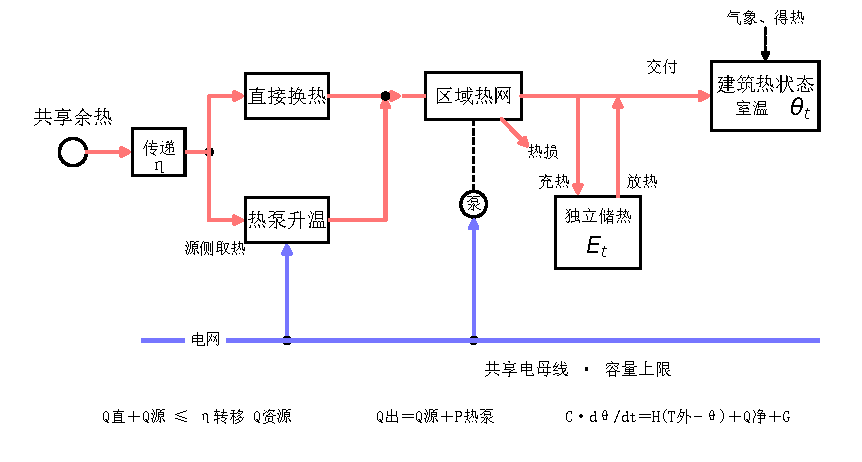
\includegraphics[width=\linewidth]{paper_r2/model_paper/source_network_load_storage_zh.pdf}
\caption{共享资源、热电网络与两类状态的统一结构。热泵源侧取热与电功分别计量；独立储热$E_t$与建筑室温$\theta_t$分别递推。各实验按配置启用模块。}
\label{fig:unified-structure}
\end{figure}

\subsection{资产容量与共享热资源}

令$k,n,g,b,s,e,t$分别表示设备、区域节点、供热温位、建筑、储热装置、管段和时段。源设备的现有、新增与退役容量共同约束各温位出力：
\begin{equation}
K_k=K_k^{\mathrm{exist}}+K_k^{\mathrm{new}}-K_k^{\mathrm{ret}},
\qquad
0\leq\sum_g Q_{k,g,t}\leq a_{k,t}K_k .
\label{eq:scoring-capacity}
\end{equation}
其中$a_{k,t}$为逐时可用率；新增上限、政策退役、启停、最小出力及爬坡由对应设备配置加载。容量约束按同一设备聚合出力，避免将不同温位视作互不占用容量的独立热源。

同一余热或可再生资源可同时连接直接换热设备与热泵，因而还需约束资源池$r$的共同取用量：
\begin{equation}
R_{r,t}^{\mathrm{use}}
=\frac{1}{\eta_r^{\mathrm{tr}}}
\left[
\sum_{k\in\mathcal D_r,g}Q_{k,g,t}
+\sum_{k\in\mathcal H_r,g}
\left(1-\frac{1}{\mathrm{COP}_{k,g,t}}\right)Q_{k,g,t}
\right]
\leq \overline R_{r,t}.
\label{eq:scoring-resource}
\end{equation}
$\eta_r^{\mathrm{tr}}\in(0,1]$为资源端至设备端的传热效率，$\mathcal D_r$与$\mathcal H_r$分别为直接换热和热泵成员。直接换热按交付量折算上游需求；热泵先扣除压缩机电功，再折算资源取热。两种路径因而共同占用同一个逐时资源预算，防止同一份余热被重复利用。资源池与成员唯一关联，资源传热、设备转换及管网输送分别核算，使瓶颈可定位到具体环节。

\subsection{设备性能域与温位适配}

通用模型以外生逐时$\mathrm{COP}$、$\mathrm{EER}$及效率描述转换，热泵与电锅炉分别满足
\begin{equation}
Q^{\mathrm{HP}}=\mathrm{COP}\,P^{\mathrm{HP}},\qquad
Q^{\mathrm{EB}}=\eta^{\mathrm{EB}}P^{\mathrm{EB}} .
\label{eq:scoring-conversion}
\end{equation}
直接热源仅接入其供水温度能够满足的温位；热泵按提升后的供热侧温位交付。温位由此同时影响资源取热、耗电与可连接用户。

厂家性能域算例进一步保留同型号、同工况的成对供热量$Q^{\mathrm{cat}}$与输入功率$P^{\mathrm{cat}}$。对相邻打印坐标分别插值，而后计算比值：
\begin{equation}
\begin{aligned}
Q_t^{\mathrm{cat}}&=\sum_i\lambda_{i,t}Q_i,\qquad
P_t^{\mathrm{cat}}=\sum_i\lambda_{i,t}P_i,\\
\mathrm{COP}_t^{\mathrm{cat}}&=\frac{Q_t^{\mathrm{cat}}}{P_t^{\mathrm{cat}}},\qquad
\lambda_{i,t}\geq0,\quad \sum_i\lambda_{i,t}=1 .
\end{aligned}
\label{eq:scoring-performance}
\end{equation}
权重由外生环境温度和出水温度的相邻坐标确定，作为预计算系数进入优化；有效域同时检查插值角点。在准入时段，固定整机算例采用声明的交付能力系数$\phi\in(0,1]$：
\begin{equation}
0\leq Q_t^{\mathrm{HP}}\leq\phi Q_t^{\mathrm{cat}},\qquad
P_t^{\mathrm{HP}}=
\frac{P_t^{\mathrm{cat}}}{\phi Q_t^{\mathrm{cat}}}Q_t^{\mathrm{HP}} .
\label{eq:scoring-duty}
\end{equation}
成对Q/P将工况变化同时传递至出力上限与单位供热耗电，使设备能力和配电占用采用一致依据。该式以理想小时占空比描述部分负荷运行，厂家表的型号、单位和工况随性能记录保存。

\subsection{节点守恒与网络物理反馈}

零失供服务下，各节点按温位逐时守恒：
\begin{multline}
\sum_{k\in\mathcal K_n}Q_{k,g,t}
+\sum_{e\in\delta^-(n)}\eta_{e,t}F_{e,g,t}
+\sum_{s\in\mathcal S_{n,g}}Q_{s,t}^{\mathrm{dis}}\\
=D_{n,g,t}+\sum_{b\in\mathcal B_{n,g}}Q_{b,t}^{\mathrm h}
+\sum_{s\in\mathcal S_{n,g}}Q_{s,t}^{\mathrm{ch}}
+\sum_{e\in\delta^+(n)}F_{e,g,t}.
\label{eq:scoring-node}
\end{multline}
$F$为管段入口功率，$\eta_{e,t}$为交付效率，故$(1-\eta_{e,t})F$为损失。$D$只表示未被建筑热状态模块覆盖、并已计入启用需求侧调整的有效固定服务，已覆盖部分以实际建筑交付量替代原负荷列。双向管段按实际方向计入，候选容量与改造状态限制输送，循环泵电耗同步进入电力账本。

有限模式网络接口将给定流量、回水温度下的双管散热、水力阻力及泵效率换算为交付效率和泵功率：
\begin{equation}
\eta_m^{\mathrm{net}}=\frac{Q_m^{\mathrm{out}}}{Q_m^{\mathrm{in}}},
\qquad
P_m^{\mathrm{pump}}=
\frac{\Delta p_m\dot m_m}{1000\,\rho\,\eta_m^{\mathrm{pump}}}.
\label{eq:scoring-network}
\end{equation}
其中压差采用Pa，质量流量采用kg/s，密度采用kg/m$^3$。求解后按运行模式的瞬时状态校核远端温度、流速、压降和泵功率；不合格模式被切除后重新求解，并保留每轮记录。这使热量平衡与工程可行性形成可追踪的反馈。

\subsection{建筑热状态与精确逐时递推}

建筑采用单状态1R1C结构\supcite{2}，将围护与换气损失、建筑蓄热及内外得热显式纳入服务约束：
\begin{align}
C_b\frac{\mathrm d\theta_b}{\mathrm dt}
&=H_b(T^{\mathrm{out}}-\theta_b)+Q_b^{\mathrm h}-Q_b^{\mathrm c}+G_b,
\label{eq:scoring-rc-cont}\\
a_b&=\exp(-H_b\Delta t/C_b),\qquad
\beta_b=(1-a_b)/H_b,\\
\theta_{b,t}
&=a_b\theta_{b,t-1}+(1-a_b)T_t^{\mathrm{out}}
+\beta_b(Q_{b,t}^{\mathrm h}-Q_{b,t}^{\mathrm c}+G_{b,t}).
\label{eq:scoring-rc}
\end{align}
$H_b$采用kW/K，$C_b$采用kWh/K，$G_b$为内部与太阳得热之和，采用kW。式\eqref{eq:scoring-rc}是区间输入保持下的精确积分，温度变量表示时段末状态；实现采用稳定指数差计算，避免小时间步下的相消误差。

逐时温度上下界直接约束状态，供热与供冷采用有限功率上界，启用互斥时以二元变量排除同楼同时冷热供给。交付功率既驱动状态，又进入式\eqref{eq:scoring-node}，预热必须占用设备及配电能力。各连续组由声明初温递推至规定终温或区间，不再叠加虚拟储热需求。同服务比较固定舒适和初末状态，以排除透支终端蓄热的收益；逐楼状态与交付量均导出复算。

\subsection{独立储热的连续性与边界}

储热与建筑状态分别建模。以下$t=1,\ldots,T$，$E_{s,0}$是首小时开始前状态。令$K_s^E$为现有与新增能量容量，$r_s$为功率能量比，单位h$^{-1}$，则
\begin{align}
E_{s,t}
&=(1-\mu_s)^{\Delta t}E_{s,t-1}
+\eta_s^{\mathrm{ch}}Q_{s,t}^{\mathrm{ch}}\Delta t
-Q_{s,t}^{\mathrm{dis}}\Delta t/\eta_s^{\mathrm{dis}},
\label{eq:scoring-storage}\\
0\leq E_{s,t}&\leq K_s^E,\qquad
0\leq Q_{s,t}^{\mathrm{ch}},Q_{s,t}^{\mathrm{dis}}\leq r_sK_s^E .
\end{align}
$\mu_s$为每小时自损失率，充、放热效率均为无量纲；严格模式以二元变量约束充放互斥。固定初态采用$E_{s,0}=f_s^{\mathrm{init}}K_s^E$，组末要求$E_{s,\mathrm{end}}\geq f_s^{\mathrm{final}}K_s^E$；循环边界连接组首与组末。容量、充放功率及温位分别限定移峰深度、持续时间与服务对象。组内状态连续递推，代表期权重仅累计费用和能量。安装容量及边界随案例登记；建筑RC及多尺度案例采用空储热集以识别建筑自身的柔性。

\subsection{共享电力与多尺度耦合}

各电驱热源、制冷设备及循环泵的功率合并为系统电负荷：
\begin{align}
P_t^{\mathrm{sys}}
&=\sum_{k,g}\frac{Q_{k,g,t}^{\mathrm{HP}}}{\mathrm{COP}_{k,g,t}}
+\sum_k\frac{Q_{k,t}^{\mathrm{EB}}}{\eta_k^{\mathrm{EB}}}
\notag\\
&\quad+\sum_k\frac{Q_{k,t}^{\mathrm c}}{\mathrm{EER}_{k,t}}
+\sum_eP_{e,t}^{\mathrm{pump}},
\notag\\
(1+\sigma)P_t^{\mathrm{sys}}&\leq a_t^{\mathrm{grid}}K^{\mathrm{grid}}.
\label{eq:scoring-electric}
\end{align}
该式对应无微电网的共享接入约束，$\sigma$为备用裕度。启用微电网时，充电增加进口需求，本地发电与放电减少进口需求，并约束进口非负。统一电负荷注册表同时服务配电约束和电量统计，重复注册或冻结后漏加负荷会直接报错。系统接入投资传递至区域设备运行，节点聚合再传递至逐楼交付与温度状态；共享上限绑定时，各建筑通过真实电力竞争发生耦合。

\subsection{经济与系统碳的共同账本}

费用和碳排采用相同物理调度量及时间权重。设$\omega_t=\pi_t w_t\Delta t$，其中$\pi_t$为情景概率、$w_t$为代表期频数权重，基本账本为
\begin{equation}
\begin{aligned}
C_0={}&\mathrm{CRF}\,I_{\mathrm{net}}+C_{\mathrm{fix}}+C_{\mathrm{event}}+C_{\mathrm{basic}}+C_{\mathrm{other}}
+\sum_t\omega_t\,\boldsymbol c_t^\mathsf T\boldsymbol x_t,\\
\mathcal E={}&\mathcal E_{\mathrm{const}}+\sum_t\omega_t\,\boldsymbol e_t^\mathsf T\boldsymbol x_t .
\end{aligned}
\label{eq:scoring-ledger}
\end{equation}
$\boldsymbol x_t$为逐时运行变量向量；费用以元、碳排以kg计。$C_{\mathrm{event}}$、$C_{\mathrm{basic}}$和$C_{\mathrm{other}}$分别汇总启停、基本电费及其他启用费用。后文采用$F_C=C_0+C_{\mathrm{carbon}}+C_{\mathrm{pref}}$、$F_E=\mathcal E$。投资扣除声明补贴后年化，设备、泵及本地供电按共同调度量计费；供热、供冷和共享电力合计碳排后施加碳帽，使经济与环境目标比较同一份服务。

地源设备逐源、逐情景累计供热取热与供冷排热，分别扣除与计入压缩机电耗；启用年度比例时检查
\begin{equation}
r_j^{\min}E_j^{\mathrm{rej}}\leq E_j^{\mathrm{ext}}
\leq r_j^{\max}E_j^{\mathrm{rej}} .
\label{eq:ground-ledger}
\end{equation}
以上约束通过统一变量与节点接口装配。网络、储热和地源模块按场景配置启用，形成面向不同服务边界的可复用模型。
